\documentclass[12pt,answers]{exam}
\usepackage[version=4]{mhchem}
\usepackage[usenames,dvipsnames]{color}
\usepackage[T1]{fontenc}
\usepackage{tikz}
\usetikzlibrary{positioning}
\usetikzlibrary{arrows}
\usetikzlibrary{shapes.multipart}
\usepackage[caption=false]{subfig}
\usepackage{tabularx,tikz}
\usepackage{graphicx}
\usepackage{color}
\usepackage{pdfpages}

\pagestyle{headandfoot}
\runningheadrule
\firstpageheader{Name: \fillin[][4cm]}{Atomic Structure Notes}{Period \fillin[][1cm]}
\runningheader{Chemistry B}{Atomic Structure}{\today}
\firstpagefooter{}{}{}
\runningfooter{Chemistry B}{Atomic Structure, Page \thepage\ of \numpages}{\today}

\begin{document}
\twocolumn
    
\begin{questions}
        
\section{Atomic Structure}

\subsection{atomic number and mass}

\question The \fillin[atomic number][4cm] is the number of \fillin[protons][3cm] in the nucleus of an atom.

\question The \fillin[mass number][3cm] is the total number of \fillin[protons][2cm] and \fillin[neutrons][2cm]in the nucleus of an atom.



\question $$\ce{^{1}_{}H}$$
What does the 1 mean?

\fillin[\# of protons and neutrons][6cm]


$$\ce{^{4}_{2}He}$$

\question What does the 4 mean? 

\fillin[\# of protons and neutrons][6cm]

\question What does the 2 mean?

\fillin[\# of neutrons][6cm]

\question $$\ce{^{7}_{3}Li}$$

How many protons does Lithium have? \fillin[3][2cm]

How many neutrons does Lithium have? \fillin[7 - 3 = 4][2cm]

\question $$\ce{^{2}_{}H}$$ based on this symbol, how many protons does Hydrogen have? \fillin[1][1cm]

How many neutrons? \fillin[1][1cm]

\subsection{The Bohr model}

\question   The Bohr Model - Bohr proposed that an atom was a nucleus with electrons "orbiting" in different \fillin[energy levels].

\question Electrons can only have certain energy values known as \fillin[energy levels]

\subsection{Electron Configuration}

\question The electrons closest to the nucleus have the \fillin[lowest] energy, while those further from away have \fillin[higher] energy.

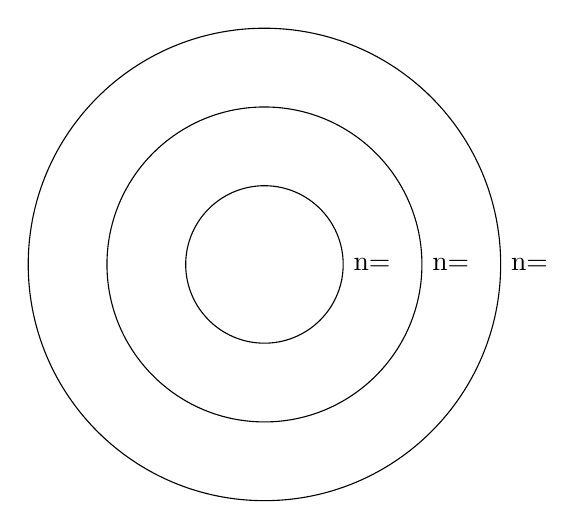
\begin{tikzpicture}
    \foreach \r/\c in {1/n=, 2/n=, 3/n=} 
    {
      \node[circle, draw, minimum size=2*\r cm,label=right:\c] {};
    }
      \end{tikzpicture}

\question draw the electron configuration for \ce{H}

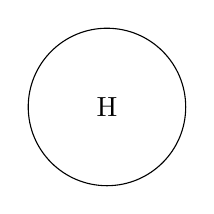
\begin{tikzpicture}
\foreach \r/\c in {1/H} {\node[circle, draw, minimum size=2*\r cm,label=center:\c] {};}
\end{tikzpicture}

\question draw the electron configuration for \ce{He}

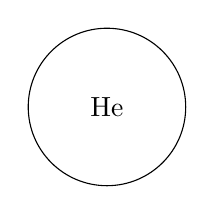
\begin{tikzpicture}
\foreach \r/\c in {1/He} {\node[circle, draw, minimum size=2*\r cm,label=center:\c] {};}
\end{tikzpicture}

\pagebreak
\question draw the electron configuration for \ce{Li}


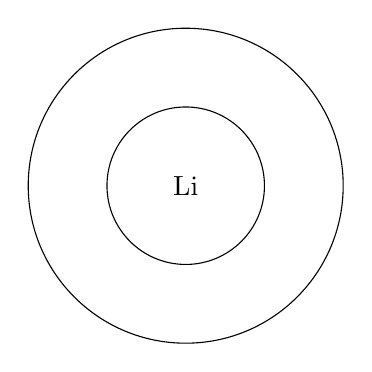
\begin{tikzpicture}
\foreach \r/\c in {1/Li, 2/ } {\node[circle, draw, minimum size=2*\r cm,label=center:\c] {};}
\end{tikzpicture}


\question draw the electron configuration for Boron \ce{B} 

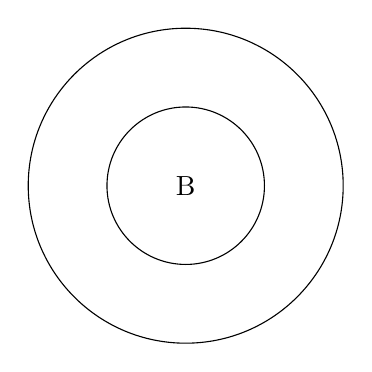
\begin{tikzpicture}
\foreach \r/\c in {1/B, 2/} {\node[circle, draw, minimum size=2*\r cm,label=center:\c] {};}
\end{tikzpicture}


\question draw the electron configuration for Carbon \ce{C} 

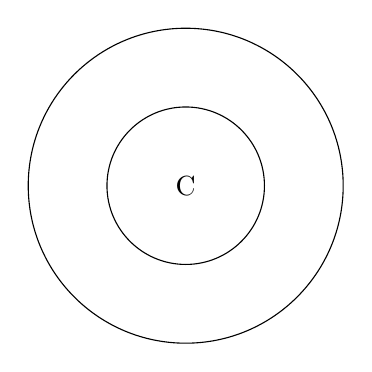
\begin{tikzpicture}
\foreach \r/\c in {1/C, 2/} {\node[circle, draw, minimum size=2*\r cm,label=center:\c] {};}
\end{tikzpicture}


\question draw the electron configuration for Nitrogen \ce{N} 

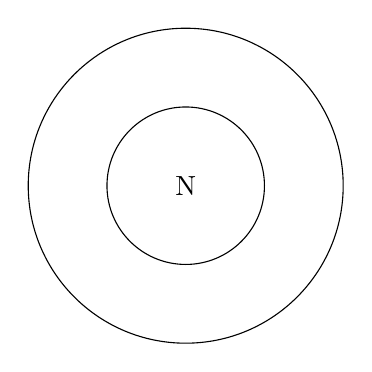
\begin{tikzpicture}
\foreach \r/\c in {1/N, 2/} {\node[circle, draw, minimum size=2*\r cm,label=center:\c] {};}
\end{tikzpicture}


\question draw the electron configuration for Oxygen \ce{O} 

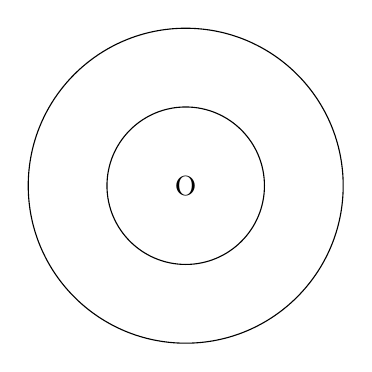
\begin{tikzpicture}
\foreach \r/\c in {1/O, 2/} {\node[circle, draw, minimum size=2*\r cm,label=center:\c] {};}
\end{tikzpicture}

\question draw the electron configuration for Flourine \ce{F} 

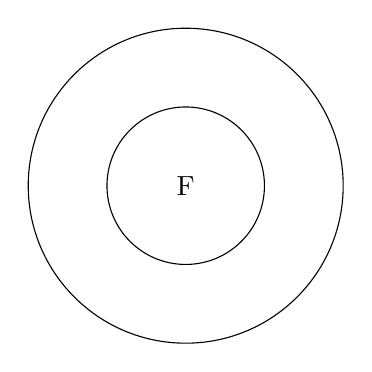
\begin{tikzpicture}
\foreach \r/\c in {1/F, 2/} {\node[circle, draw, minimum size=2*\r cm,label=center:\c] {};}
\end{tikzpicture}


\question draw the electron configuration for Neon \ce{Ne} 

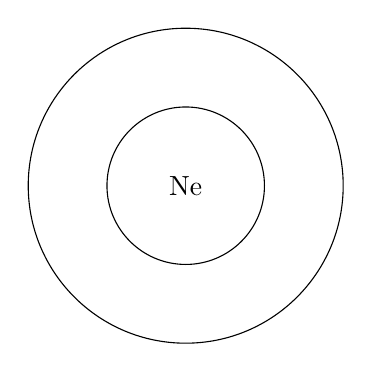
\begin{tikzpicture}
\foreach \r/\c in {1/Ne, 2/} {\node[circle, draw, minimum size=2*\r cm,label=center:\c] {};}
\end{tikzpicture}

\end{questions}

\end{document}